\documentclass{article}
\usepackage{graphicx} % Required for inserting images
\usepackage{amsmath}
\usepackage{caption}
\usepackage{amssymb}
\usepackage{array} % for tables
\usepackage{amsfonts}
\usepackage{tabularx}
\usepackage{geometry} % for tables and graphs 
\usepackage{hyperref}
\usepackage{float}
\usepackage{pgfplots} % for graphs in line
\usepackage{longtable}
\usepackage{tikz}
\usetikzlibrary{trees,positioning,arrows}


\geometry{a4paper, margin=1in}
\pgfplotsset{compat=1.18}

% this document is a re-written provision of the solutions for the midterm 
\begin{document}

\section*{Q1: on strict dominance}
\subsection*{(a) Payoff Matrix}

\[
\begin{array}{c|cc|cc}
    & \multicolumn{2}{c|}{P2 \text{ if } P1 = T} & \multicolumn{2}{c}{P2  \text{ if } P1 = B} \\
    & L & R & L & R  \\
    \hline
    X & (2,2,0) & (1,1,2) & (1.5,2,0) & (0,1,2)  \\
    Y & (3,1,2) & (1,2,0) & (2,1,2) & (0,2,0)  \\
    Z & (1.5,0,1) & (7,0,1) & (1,0, 1.5) & (4,0,1.5)  \\
\end{array}
\]
\\

$\rightharpoondown$ \textit{\textbf{for pure dominant strategies:}}
\begin{itemize}
    \item No pure dominant strategy for Player 3.
    \item No pure dominant strategy for Player 2.
    \item However, for Player 1, all payoffs in the table where \( P_1 \) chooses \( s_2 = T \) have strictly larger values.
    \item Therefore, Player 1 has a \textbf{pure dominant strategy}.
    \item In part (b), we will see the strictly dominated pure strategy \( s_1 = B \) will be eliminated.
\end{itemize}
\vspace{2mm}
\hspace{4mm}
$\rightharpoondown$ \textit{\textbf{formixed dominant strategies:}}
\begin{itemize}
    \item To analyze mixed strategies, compare mixed strategy payoffs in a finite number of contexts, considering only pure strategy profiles.
    \item Evaluate mixed strategy dominance in a game \textbf{only} after eliminating strictly dominated pure strategies.
\end{itemize}
\\

For \( P_2 \), we set expected payoffs:

\[
2p_X + 1p_Y + 0p_Z = 1p_X + 2pY + 0p_Z
\]
\[
2p_X + p_Y = 2p_Y
\]
\[
p_X = p_Y
\]
\\
Now we look at the \textbf{expected pay off functions} for the utility of players 2 and 3: 
\\

\[
E_{\sigma}(u_2(\sigma,L)) = \frac{1}{2} \cdot 2 + \frac{1}{2} \cdot 1 + (0 \cdot 0)
\]

\[
E_{\sigma}(u_2(\sigma,R)) = \frac{1}{2} \cdot 1 + \frac{1}{2} \cdot 2 + (0 \cdot 0)
\]
\\ 
\textbf{For domination of P2:}
\begin{itemize}
    \item If probability mass is more heavily on \( P_3 \) choosing \( X \), then \( R \) would dominate.
    \item If probability mass is more on \( P_3 \) choosing \( Y \), then \( L \) would dominate.
\end{itemize}


\[
E_{\sigma}(u_3(\sigma,X)) = \frac{1}{2} \cdot 0 + \frac{1}{2} \cdot 2 = 1 
\]

\[
E_{\sigma}(u_3(\sigma,Y)) = \frac{1}{2} \cdot 2 + \frac{1}{2} \cdot 0 = 1
\]

\[
E_{\sigma}(u_3(\sigma,Z)) = \frac{1}{2} \cdot 1 + \frac{1}{2} \cdot 1 = 1
\]

\vspace{2mm}
\textbf{For domination of P3:}
\begin{itemize}
    \item If probability mass is more heavily on \( P_2 \) choosing \( L \), then \( Y \) would dominate.
    \item If probability mass is more on \( P_2 \) choosing \( R \), then \( X \) would dominate for P3
    \item Note when we compare with the choice of Z, we always yield a payoff of 1, as well, so we can ignore it in terms of comparison. 
\end{itemize}
\vspace{2mm}

\textit{\textbf{Takeaway:}}
\begin{itemize}
    \item If \( p_X > \frac{1}{2} \), then \( \sigma_2 = \{L\} \); if \( p_X < \frac{1}{2} \), then \( \sigma_2 = \{R\} \) (and \( p_Z = 0 \)).
    \item If \( p_\ell > \frac{1}{2} \), then \( \sigma_3 = \{Y\} \); if \( p_\ell < \frac{1}{2} \), then \( \sigma_3 = \{X\} \).
    \item A mixed strategy with \( z \) is only possible when \( p_\ell = p_R = \frac{1}{2} \).
    \item So a mixed, dominated strategy occurs when:
\end{itemize}

\[
\sigma_3 = \left( >\frac{1}{2}, <\frac{1}{2}, 0 \right) \Rightarrow \text{Then player 2 chooses } L
\]

\[
\sigma_3 = \left( <\frac{1}{2}, >\frac{1}{2}, 0 \right) \Rightarrow \text{Then player 2 chooses } R
\]

\[
\sigma_2 = \left( >\frac{1}{2}, <\frac{1}{2} \right) \Rightarrow \text{Then } P_3 \text{ chooses } Y
\]

\[
\sigma_2 = \left( <\frac{1}{2}, >\frac{1}{2} \right) \Rightarrow \text{Then } P_3 \text{ chooses } X
\]

\[
\text{When } \sigma_2 = \left(\frac{1}{2}, \frac{1}{2} \right) \Rightarrow \text{Indifferent to mixed strategy}
\]

\subsection*{(b) Iterated deletion}

We eliminate \( S_1 = \{B\} \) using iterated deletion. No pure dominant strategy remains. So, the only never best response (NBR) is: \( S_1 = \{B\} \). This is dropped.

\subsection*{(c) Nash equilibria}
Using \textbf{best response correspondence} we have the following for pure nash equilibrium:
\[
BR_2(X) = L, \quad BR_2(Y) = L, \quad BR_2(Z) = \{L, R\}
\]

\[
BR_3(L) = Y, \quad BR_3(R) = X
\]
\vspace{2mm}

There is no pure Nash equilibrium that we can see from the best response correspondences, so we analyze the mixed strategy case.
\vspace{2mm}
\[
\text{when } \sigma_{3a} = \left( >\frac{1}{2}, <\frac{1}{2}, 0 \right) \implies \{(BR_2(X) = L), (BR_2(Y) = L), (BR_2(Z) = L)\}
\]
\[
\text{when } \sigma_{3b} = \left( <\frac{1}{2}, >\frac{1}{2}, 0 \right) \implies \{(BR_2(X) = R), (BR_2(Y) = R), (BR_2(Z) = R)\}
\]
\[
\text{when } \sigma_{2a} = \left( >\frac{1}{2}, <\frac{1}{2}, \right) \implies \{(BR_3(L) = Y), (BR_3(R) = Y)\}
\]
\[
\text{when } \sigma_{2b} = \left( <\frac{1}{2}, >\frac{1}{2} \right) \implies \{(BR_3(L) = X), (BR_3(R) = X)\}
\]

\[
(\sigma_{3a}, \sigma_{3b}) = (X, Y, Z) = \left(\frac{1}{2}, \frac{1}{2}, 0\right), \quad (\sigma_{2a}, \sigma_{2b}) =  (L, R) = \left(\frac{1}{2}, \frac{1}{2}\right)
\] \\

\hspace{3mm}
\vspace{2mm}
Mixed strategies require specific conditions where probabilities sum to 1. \\
\vspace{2mm}
In the \textbf{mixed strategy case}, we can more formula characterize the process to find the nash equilibrium where:

\[ L \text{ has probability} = q \quad 
R \text{ has probability} = (1-q)
\]

\[ X \text{ has probability} = p_1 \quad 
Y \text{ has probability} = p_2 \quad 
Z \text{ has probability} = (1-p_{1}-p_{2})
\]
so we solve for the probability, $p$:
\[
u_2(L,X) = u_2(R,X) \quad u_3(y,X) = u_3(y,Y) = u_3(y,Z)
\]
\[
\text{so:} 2\cdot p_1 + 1 \cdot p_1 + 0\cdot (1-p_1 - p_2) = 1\cdot p_1 + 2 \cdot p_2 + 0 
\]

\[
\implies p^{*}_1 = p^{*}_2 = \frac{1}{2}
\]

now solve for the probability, $q$ (to find the mixed nash), where 
\[
q_1\cdot 0 + (1- q_1) \cdot 2 = 2 \cdot q_1  - (1-q_1) \cdot 0 = 1 \cdot q_1 + (1-q_1) \cdot 1
\]
\[
2 - q_1\cdot 2  = 2 \cdot q_1  = 1
\]
\[ \implies \frac{1}{4} = q^{*}_1 \]

\begin{align*}
    \sigma_3 = (X, Y, Z) &= \left(\frac{1}{2}, \frac{1}{2}, 0\right), \\
    \sigma_2 =  (L, R) &= \left(\frac{1}{4}, \frac{3}{4}\right).
\end{align*}

\section*{Q2: Profit max game with bayesian analysis}

\subsection*{(a) Game set up}
Here we start with the information we know about each player: 
\begin{align*}
    P_1 & \to c_1 + q_1, \quad p_1 \in \{3,5\} \\
    P_2 & c_2^H, c_2^L \text{ with probabilities } 
\end{align*}

\[
c_2^H = 4 \text{ with } \pi = \frac{4}{5} =  (1 - \theta) \text{ and } \quad c_2^L = 1 \text{ with } \pi = \frac{1}{5} = \theta
\]

\vspace{2mm}

Only Player 1 is given \( p_2 \in \{3, 5\} \), but Player 2 does not have a predefined set of prices. The expected value, then for player is calculated as a function of the probabilities (given) for both \textit{low cost} $c_2^L$ and \textit{high cost} $c_2^H$ scenarios:

\begin{align*}
    E[c_2] &= \frac{1}{5} \cdot 3 + \frac{4}{5} \cdot 4 \\
         &= 3.4.
\end{align*}

\begin{itemize}
    \item If \( C_x \leq C_y \), then \( C_x \) gets \( Q \) (\( Q = 10 \)).
    \item If \( C_x = C_y \), then \( C_x \) gets \( \frac{1}{2} Q \) (\( Q/2 = 5 \)) and \( C_y \) gets \( \frac{1}{2} Q \) (\( = 5 \)).
\end{itemize}

\[
\Pi (\text{profits}): \quad \Pi_i = (p_i - c_i)(Q_i)
\]
\vspace{2mm}
\textbf{Note:} Only Player 1 is given \( p_2 \in \{3,5\} \) and Player 2 is NOT given a set of prices to choose from in the game setup. But, with the profit function \( f(x) \), you say "a firm \( i \) chooses \( p_i \), \( c_i \) is MC", and so on. Therefore, I am going to assume Player 2 also chooses a price, where \( p_2 \in \{3,5\} \), the same restriction as Player 1. 
\vspace{2mm}

\textbf{Incomplete information:} Payoff functions are UNKNOWN, \( P_2 \) type is unknown to Player 1.

\[
P_1 \to \text{Strat:} \quad \{3,5\}
\]

\[
\text{Payoff:} 
\begin{cases}
    (3 - 2)(10) = 10, & \text{if } p_2 > 3 \\
    (3 - 2)(5) = 5, & \text{if } p_2 = 3 \\
    (3 - 2)(0) = 0, & \text{if } p_2 < 3
\end{cases}
\]

\[
\text{Payoff:}
\begin{cases}
    (5 - 2)(10) = 30, & \text{if } p_2 \geq 5 \\
    (5 - 2)(5) = 15, & \text{if } p_2 = 5 \\
    (5 - 2)(0) = 0, & \text{if } p_2 < 5
\end{cases}
\]

\textbf{Recall:} For \( P_2 \), strategy \( \{3,5\} \) with \( c_2 = \theta + 4(1 - \theta) \), so:

\[
c_2 = 4 - 3\theta
\]

\textbf{Solving:}

\[
\text{When } 4 - 3\theta > 3 \quad \implies -3\theta > -1 \quad \implies \theta < \frac{1}{3}
\]

So \( \theta < \frac{1}{3} \) if \( P_2 \) chooses \( p_1 = 3 \).

\[
\theta = \frac{1}{3}, \quad \mathbb{E}[u_2(3)] = 10
\]

\[
\theta = \frac{1}{3}, \quad \mathbb{E}[u_2(3)] = 5
\]

\[
\theta = \frac{1}{3}, \quad \mathbb{E}[u_2(3)] = 0
\]

\textbf{Next case:}

\[
\text{When } 4 - 3\theta > 5 \quad \implies -3\theta > -1 \quad \imples \theta < -\frac{1}{3}
\]
\textbf{But you can't have negative probabilities} so we ignore this case. We revisit the payoff tables for a high cost and low cost game
\[
\begin{array}{c|cc}
    & p_2 = 3 & p_2 = 5 \\
    \hline
    p_1 = 3 & (5,-5) & (10,0) \\
    p_1 = 5 & (0,-10) & (15,5) \\
\end{array}
\]

\[
c_2 = c^H = (1 - \theta)
\]

\[
\begin{array}{c|cc}
    & p_2 = 3 & p_2 = 5 \\
    \hline
    p_1 = 3 & (5,10) & (10,0) \\
    p_1 = 5 & (0,40) & (15,80) \\
\end{array}
\]

\[
c_2 = C^L = (\theta)
\]

\textbf{High Cost Game}
\begin{align*}
    3,3 &\to 1 \to (3 - 2)(5) = 5 \\
    &\to 2 \to (3 - 4)(5) = -5
\end{align*}

\begin{align*}
    3,5 &\to 1 \to (3 - 2)(0) = 10 \\
    &\to 2 \to (5 - 5)(10) = 0
\end{align*}

\begin{align*}
    5,5 &\to 1 \to (5 - 2)(5) = 15 \\
    &\to 2 \to (5 - 4)(5) = 5
\end{align*}

\begin{align*}
    5,3 &\to 1 \to (5 - 2)(10) = 0 \\
    &\to 2 \to (3 - 4)(10) = -10
\end{align*}

\textbf{Low Cost Game}
\begin{align*}
    3,3 &\to 1 \to (3 - 2)(5) = 5 \\
    &\to 2 \to (3 - 1)(5) = 10
\end{align*}

\begin{align*}
    3,5 &\to 1 \to (3 - 2)(0) = 10 \\
    &\to 2 \to (5 - 1)(10) = 0
\end{align*}

\begin{align*}
    5,5 &\to 1 \to (5 - 2)(5) = 15 \\
    &\to 2 \to (5 - 1)(5) = 20
\end{align*}

\begin{align*}
    5,3 &\to 1 \to (5 - 2)(0) = 0 \\
    &\to 2 \to (5 - 1)(10) = 90
\end{align*}

\subsection*{(b) Game of imperfect information}
Nature determines the type of \textbf{Player 2} with probabilities:
\[
\theta, (1 - \theta) \quad \text{for low and high cost types}
\]

This can be represented as:
\[
\hat{\Gamma}_n = \left[ I, \{ I_i \}, \{ u_i(\sigma) \} \right]
\]

% remake in tikz with time 
\begin{center}
 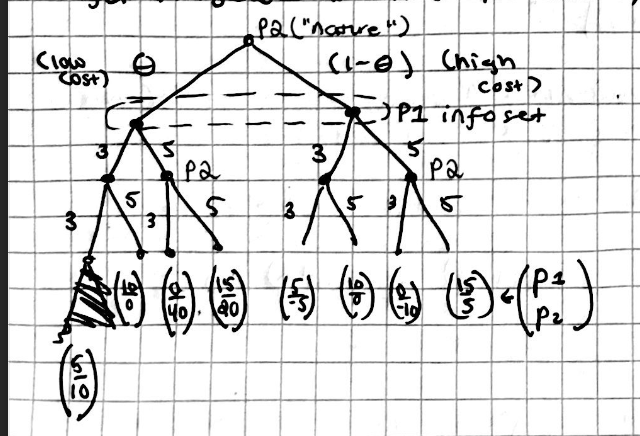
\includegraphics[width=.75\linewidth]{images/Screenshot 2025-03-02 at 19.07.23.png} 
\end{center}

\subsection*{(c) Find BNE}
\begin{itemize}
    \item No pure strategy dominance for \( P_1 \).
    \item In the low-cost game, \( s_2 = 3 \) is dominant.
    \item In the high-cost game, \( s_2 = s_5 \) is always dominant, in subgames.
    \item \textit{Note:} I tried to take the first derivative of the expected utility with respect to q, p (the probabilities) and I got a value over 1, so I was not able to use this approach. 
\end{itemize}

\begin{enumerate}
    \item In the low-cost game, \( P_2 \) best response (BR) is:
    \[
    BR_2(3) = 3, \quad BR_2(5) = 3
    \]
    So, the dominant strategy for \( P_2 \) in the low-cost game is to play 3.
    
    \item In the high-cost game, \( P_2 \) has no dominant strategy.
    
    \item Payoffs are the same for \( P_1 \) in all games.
\end{enumerate}
\vspace{2mm}
However, the expected utility \( E(u_i) \) for \( i=1 \) when \( S = \{5\} \) and with an unknown \( \theta \), Player 1 always chooses \( S_1 = \{5\} \) (refer to part (a) for calculation).

\[
\theta = \frac{1}{3}
\]

Then, the expected cost:

\[
E[c_2] = \theta(1) + (1-\theta)(4)
\]

\[
= \frac{1}{3} + \frac{8}{3}
\]

\[
= \frac{9}{3} = 3
\]
\vspace{2mm}
When \( \theta = \frac{1}{3} \), the expected cost for \( P_2 \) is 3. Also, \( E[u_2(s_2 = 5)] = 10 \). 
\vspace{2mm}
Thus, the \textbf{BNE} occurs where \( P_2 \) will always choose \( S_2 = \{5\} \) based on the expected value.

\[
\text{Bayesian Nash} = \left\{ \frac{1}{3}, \frac{2}{3} \right\} = \{ \sigma_2 \} = \{ 5, 5 \} \quad \text{for } (P_1, P_2).
\]

\section*{Q3: Weak pure bayesian nash (WPBE)}


% remake in tikz with time 
\begin{center}
 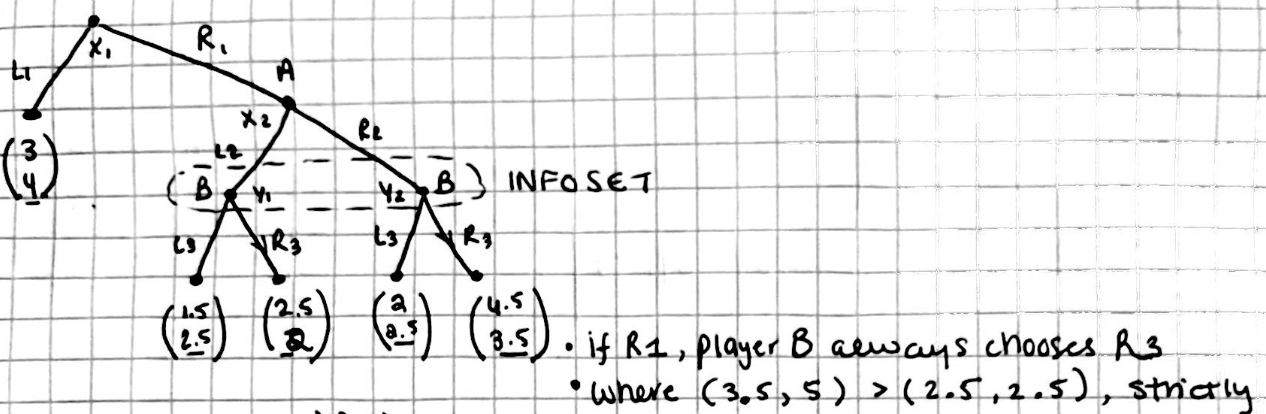
\includegraphics[width=.75\linewidth]{images/Screenshot 2025-03-02 at 19.20.19.png} 
\end{center}


\subsection*{(a) Find all NE}
For Player A, considering strategies:
\[
S_A = \{L_1, (R_1, R_2), (R_1, L_2)\}
\]
For Player B, considering strategies:
\[
S_B = \{R_3, L_3\}
\]

To find Nash equilibrium, we start with \textbf{backward induction} and dominance.

\begin{itemize}
    \item Notice that \( S_A = \{(R_1, L_2)\} \) is strictly dominated by \( (R_1, R_2) \) and \( L_1 \).
    \item Therefore, Player A will not play \( (R_1, L_2) \).
    \item If this is the case, the remaining strategies for \( S_A \) are \( \{L_1, (R_1, R_2)\} \).
\end{itemize}

Using \textbf{backward induction} at Player B's information set:

\begin{itemize}
    \item At \( S_B(L_3, R_3) \), the two nodes in \( S_B \) for Player B indicate that starting at \( (L_3, R_3) \), Player B will choose \( R_3 \).
    \item Thus, set aside and eliminate \( (L_3, L_3) \) payoff.
    \item At \( y_2 \), assume Player B would choose \( R_3 \), eliminating \( (L_2, S_3) \) payoff.
    \item Now for Player A:
    \[
    (4.5, 3.5), (1.5, 2.5) \impliedby (L2, R2)
    \]
    \item Since \( 3.5 \) is less than the payoff \( 4.5 \), Player A chooses the latter, \( R_2 \), eliminating \( L_2 - R_3 \) payoff.
    \item At Player A's initial decision node, they choose between \( L_1 \) and \( R_1 \).
    \item Since \( 3.4 \) is less than \( 4.5 \), Player A selects \( R_1, R_2 \).
\end{itemize}

By \textbf{backward induction}, the highest payoff will be:
\[
S_A = \{R_1, R_2\}
\]
\[
S_B = \{R_3\}
\]

To confirm this as a Nash equilibrium, we verify the \textbf{subgame perfect Nash equilibrium (SPNE)}:
\[
\{(R_1, R_2), (R_3)\} \quad \text{and} \quad \{(L_1, L_3)\} \quad \text{for both subgames in this game.}
\]

\subsection*{(b) all weak PBEs}

All weak PBEs $\Rightarrow$ where weak PBEs do \textbf{not} need to be subgame perfect, but we need the strategy profile of both players to be \textbf{sequentially rational}, given belief system $\mu$. We need to follow the belief system derived from the strategy profile through \textbf{Bayes' Rule} when possible.

\[
\Rightarrow \text{recall not all weak PBEs are Nash Eq (and vice versa)}
\]

When A is indifferent between $L_1, R_1$:
\begin{itemize}
    \item Assign $\sigma_{L_3} = (1 - \sigma_{R_3})$ for probability of Player B choosing $L_3, R_3$ at info set.
    \item So $\sigma_{L_3} = \sigma_{R_3}$ (for nonrandom).
\end{itemize}

\[
1.5(1 - \sigma_{R_3}) + 2.5\sigma_{R_3} = 2(1 - \sigma_{R_3}) + 4.5\sigma_{R_3}
\]

\[
1.5 - 1.5\sigma_{R_3} + 2.5\sigma_{R_3} = 2 - 2\sigma_{R_3} + 4.5\sigma_{R_3}
\]

\[
1.5 - \sigma_{R_3} = 2 - 2\sigma_{R_3} + 4.5\sigma_{R_3}
\]

\[
-2 + 1\sigma_{R_3} = -2 + 3.5\sigma_{R_3}
\]

\[
-2 / 3.5 = \sigma_{R_3}
\]

\[
-2 / 4.5 = \sigma_{R_3} \Rightarrow \text{negative probability} \quad \textbf{(impossible)}
\]

\textbf{Since $L_2$ is strictly dominated, it is never preferred.}

\vspace{1em}

Let’s say $M_A =$ Player B's belief:

\[
\{\sigma_{L_1}, \sigma_{R_1 R_2}, \sigma_{R_1 R_3}\} = \text{probability Player A plays} \{L_1, R_1 R_2, R_1 R_3\}
\]

\begin{itemize}
    \item $\mu_A(R_1) \Rightarrow$ already solved for above $\Rightarrow$ \textbf{improbable} $= 0$
    \item $\mu_A(R_0) = \mu_A$ needs to be solved for
\end{itemize}

\[
\mu_A(L_1 | C_{R_3}) = 1/2
\]

\[
\mu_A(C_{R_3}) = \frac{\text{Pr}(L_1 | C_{R_3})}{\text{Pr}(R_1 | C_{R_3}) + \text{Pr}(L_1 | C_{R_3})}
\]

\[
2.5 \geq \mu_A(2) + (1 - \mu_A)3.5
\]

\[
2.5 = \theta \mu_A + 3.5 - 3.5\mu_A
\]

\[
-3.5 = -1.5\mu_A
\]

\[
-1 / -1.5 = \mu_A
\]

\[
2/3 = \mu_A
\]

\[
\Rightarrow \text{so when } \mu_A \leq 2/3, \text{ Player B plays } L_3 \text{ in response to A.}
\]

\[
\Rightarrow \text{so unique WPBE} \Rightarrow (\sigma_0, \sigma_1, \sigma_2) = \left( \frac{2}{3}, 0, \frac{1}{3} \right)
\]

\[
= \{(L_1, L_3), (R_1, L_3), (R_1, R_3)\}
\]

\subsection*{(c) weak PBEs and sequential rationality}

The answer is \textbf{no}. By definition, weak PBEs require sequential rationality given $\mu$, at all information sets. A sequential equilibrium requires that (a) the strategy profile, $\sigma$ is sequentially rational, given $\mu$ and (b) the sequence of mixed strategies converge - or is consistent. Therefore beliefs must converge and are derived via the Bayes' Rule.  
\vspace{2mm}
\begin{center}
    \textbf{all sequential equilibrium are weak PBE}
\end{center}

\end{document}